\documentclass[presentation]{beamer}

\usepackage{tikz}
\usetikzlibrary{positioning,calc}
\usetikzlibrary{shapes.geometric}
\usetikzlibrary{backgrounds}% only to show the bounding box
\usetikzlibrary{shapes,arrows}
\usepackage{pgfplots}
\usepackage{pgfplotstable}
\usetikzlibrary{pgfplots.groupplots}
\pgfplotsset{compat=1.12}

\pgfplotsset{every axis legend/.style={
    cells={anchor=west},
    inner xsep=3pt,inner ysep=2pt,nodes={inner xsep=4pt, inner
      ysep=2pt, text depth=0.15em},
    anchor=north east,
    shape=rectangle,
    at={(1, 1)}
    }
  }

\pgfplotsset{
    compat=newest,
    /pgfplots/legend image code/.code={%
        \draw[mark repeat=2,mark phase=2,#1]
            plot coordinates {
                (0cm,0cm)
                (0.5cm,0cm)
                (1.0cm,0cm)%
            };
    },
}
\usepackage{appendixnumberbeamer}
\usepackage{amsmath}
\usepackage{xcolor}
\date{3rd March 2017}
\usetheme{firedrake}

\definecolor{black}{rgb}{0,0,0}
\definecolor{orange}{rgb}{0.9019607843137255, 0.6235294117647059, 0}
\definecolor{blue}{rgb}{0.33725490196078434, 0.7058823529411765,
  0.9137254901960784}
\definecolor{green}{rgb}{0,0.6196078431372549, 0.45098039215686275}
\definecolor{yellow}{rgb}{0.9411764705882353, 0.8941176470588236,
  0.25882352941176473}
\definecolor{oblue}{rgb}{0, 0.4470588235294118, 0.6980392156862745}
\definecolor{oorange}{rgb}{0.8352941176470589, 0.3686274509803922, 0}
\definecolor{pink}{rgb}{0.8, 0.4745098039215686, 0.6549019607843137}
\pgfplotscreateplotcyclelist{decent cycle}{%
  {black, mark=diamond*, mark options={fill=black},
    mark size=2pt},
  {orange, mark=*, mark options={fill=orange},
    mark size=2pt},
  {blue, mark=square*, mark options={fill=blue},
    mark size=2pt},
  {green, mark=triangle*, mark options={fill=green},
    mark size=3pt},
  {black, mark=diamond*, mark options={fill=black},
    mark size=2pt},
  {orange, mark=*, mark options={fill=orange},
    mark size=2pt},
  {blue, mark=square*, mark options={fill=blue},
    mark size=2pt},
  {green, mark=triangle*, mark options={fill=green},
    mark size=3pt},
}

\pgfplotsset{
  decent/.style={
    cycle list name=decent cycle,
  }
}
\renewcommand{\vec}[1]{\ensuremath{\boldsymbol{#1}}}
\newcommand{\ddt}[1]{\frac{\partial #1}{\partial t}}
\newcommand{\zhat}{\hat{\vec{z}}}
\newcommand{\W}{\ensuremath{\mathbb{W}}}

\DeclareMathOperator{\grad}{grad}
\let\div\relax
\DeclareMathOperator{\div}{div}
\DeclareMathOperator{\curl}{curl}
\newcommand{\vsubset}[1]{\rotatebox[origin=c]{90}{\ensuremath{\subset}}}
\author{Lawrence Mitchell\inst{1}}
\institute{\inst{1}Departments of Computing and Mathematics, Imperial College London}
\title{z-layers, oh noes}

\graphicspath{{./\jobname.figures/}}

\newcommand{\arxivlink}[2]{%
  \href{http://www.arxiv.org/abs/#1}%
  {{\small\texttt{arXiv:\,#1\,[#2]}}}%
}
\usepackage[url=false,
            doi=true,
            isbn=false,
            style=authoryear,
            firstinits=true,
            uniquename=init,
            backend=biber]{biblatex}

\setbeamertemplate{bibliography item}{}
\renewcommand{\bibfont}{\footnotesize}
\addbibresource{references.bib}

\setlength{\bibitemsep}{1ex}

\renewbibmacro{in:}{}
\DeclareFieldFormat[article]{volume}{\textbf{#1}}
\DeclareFieldFormat{doi}{%
  doi\addcolon%
  {\scriptsize\ifhyperref{\href{http://dx.doi.org/#1}{\nolinkurl{#1}}}
    {\nolinkurl{#1}}}}
\AtEveryBibitem{%
\clearfield{pages}%
\clearfield{issue}%
\clearfield{number}%
}

\usepackage{minted}

\begin{document}

\begin{frame}
  \frametitle{First: a warning}

  How much halo do you need to compute (redundantly) residuals for
  partially discontinuous fields?

  Answer, quite a lot!

  For DG fields, if you own a cell, you need closure(support(cone(cell)))

  For HDiv fields, if you own a face, you need
  closure(support(cone(support(face))))

  Perhaps do non-redundant compute?
\end{frame}

\begin{frame}
  \frametitle{z-layers}

  Around steep topography, might want to use z-layers rather than
  $\sigma$ coordinates.

  What does this mean for the data model?

  Mostly the core computational aspects remain unchanged.

  But I need to keep track of more things.

  In particular, the layer number is now variable

  In fact, it is \emph{entity}-dependent
\end{frame}

\begin{frame}[plain]
  \begin{columns}
    \begin{column}{\textwidth}
      \only<1>{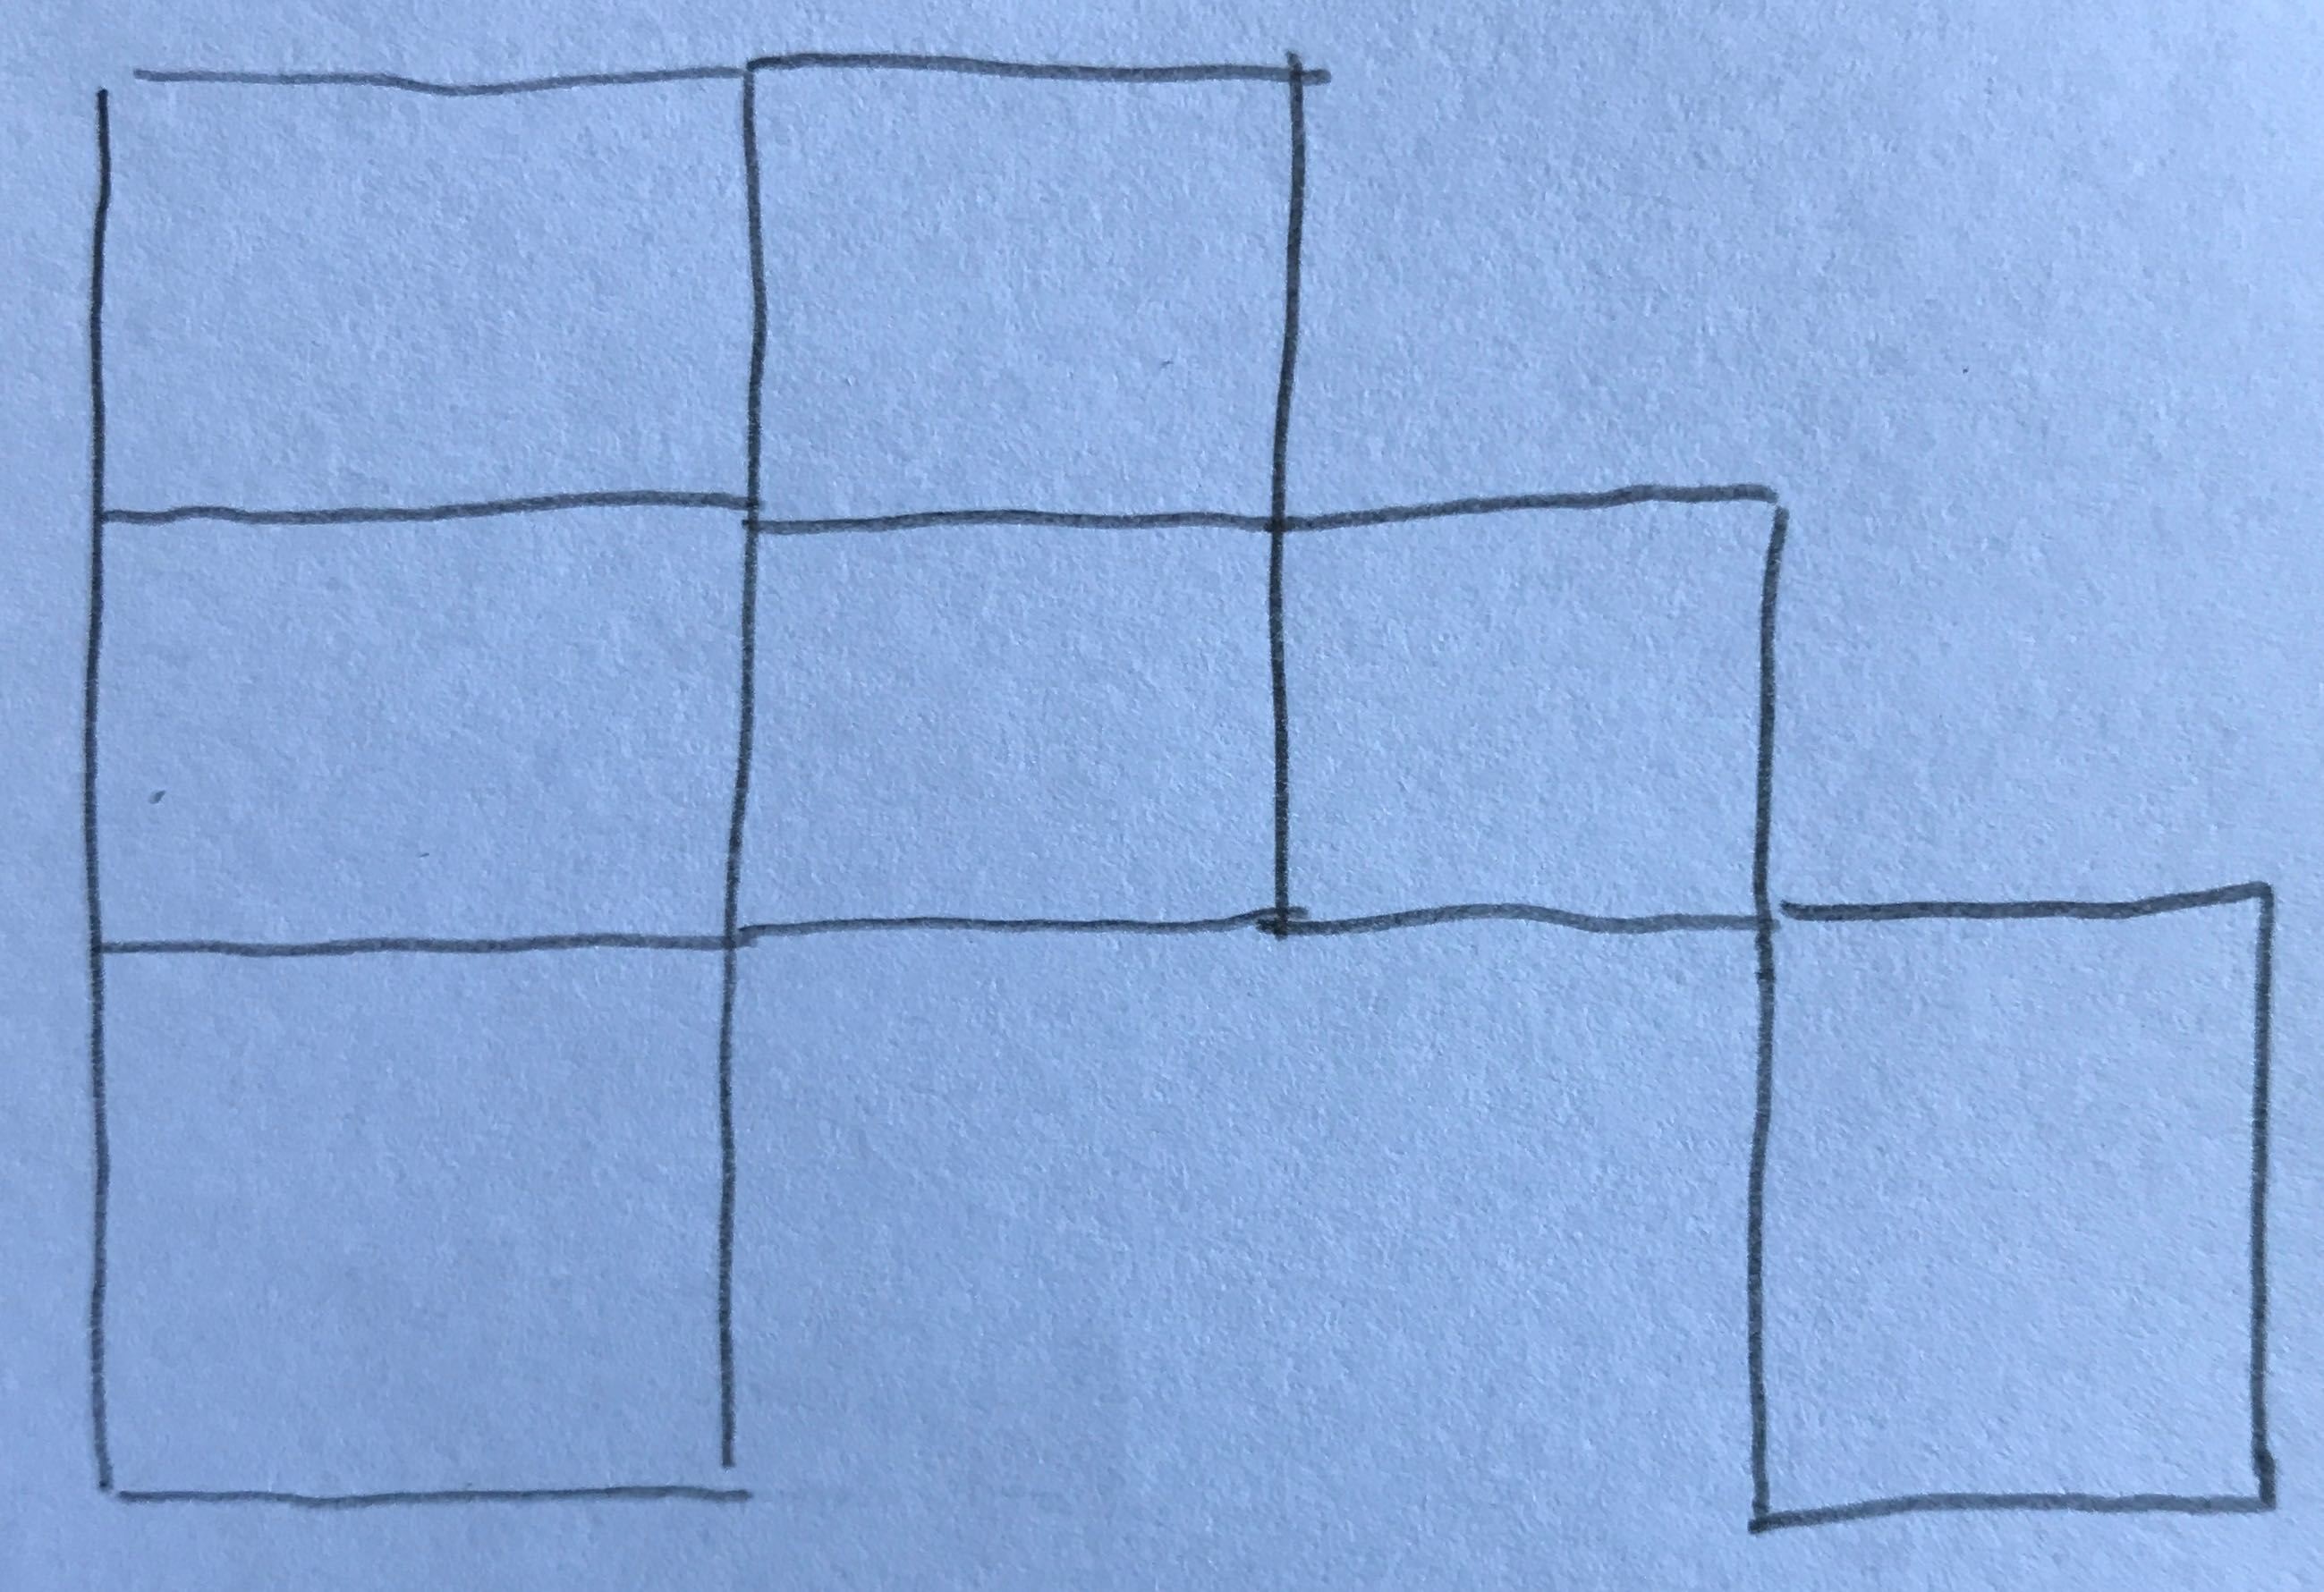
\includegraphics[width=\textwidth]{topology-2d}}
      \only<2>{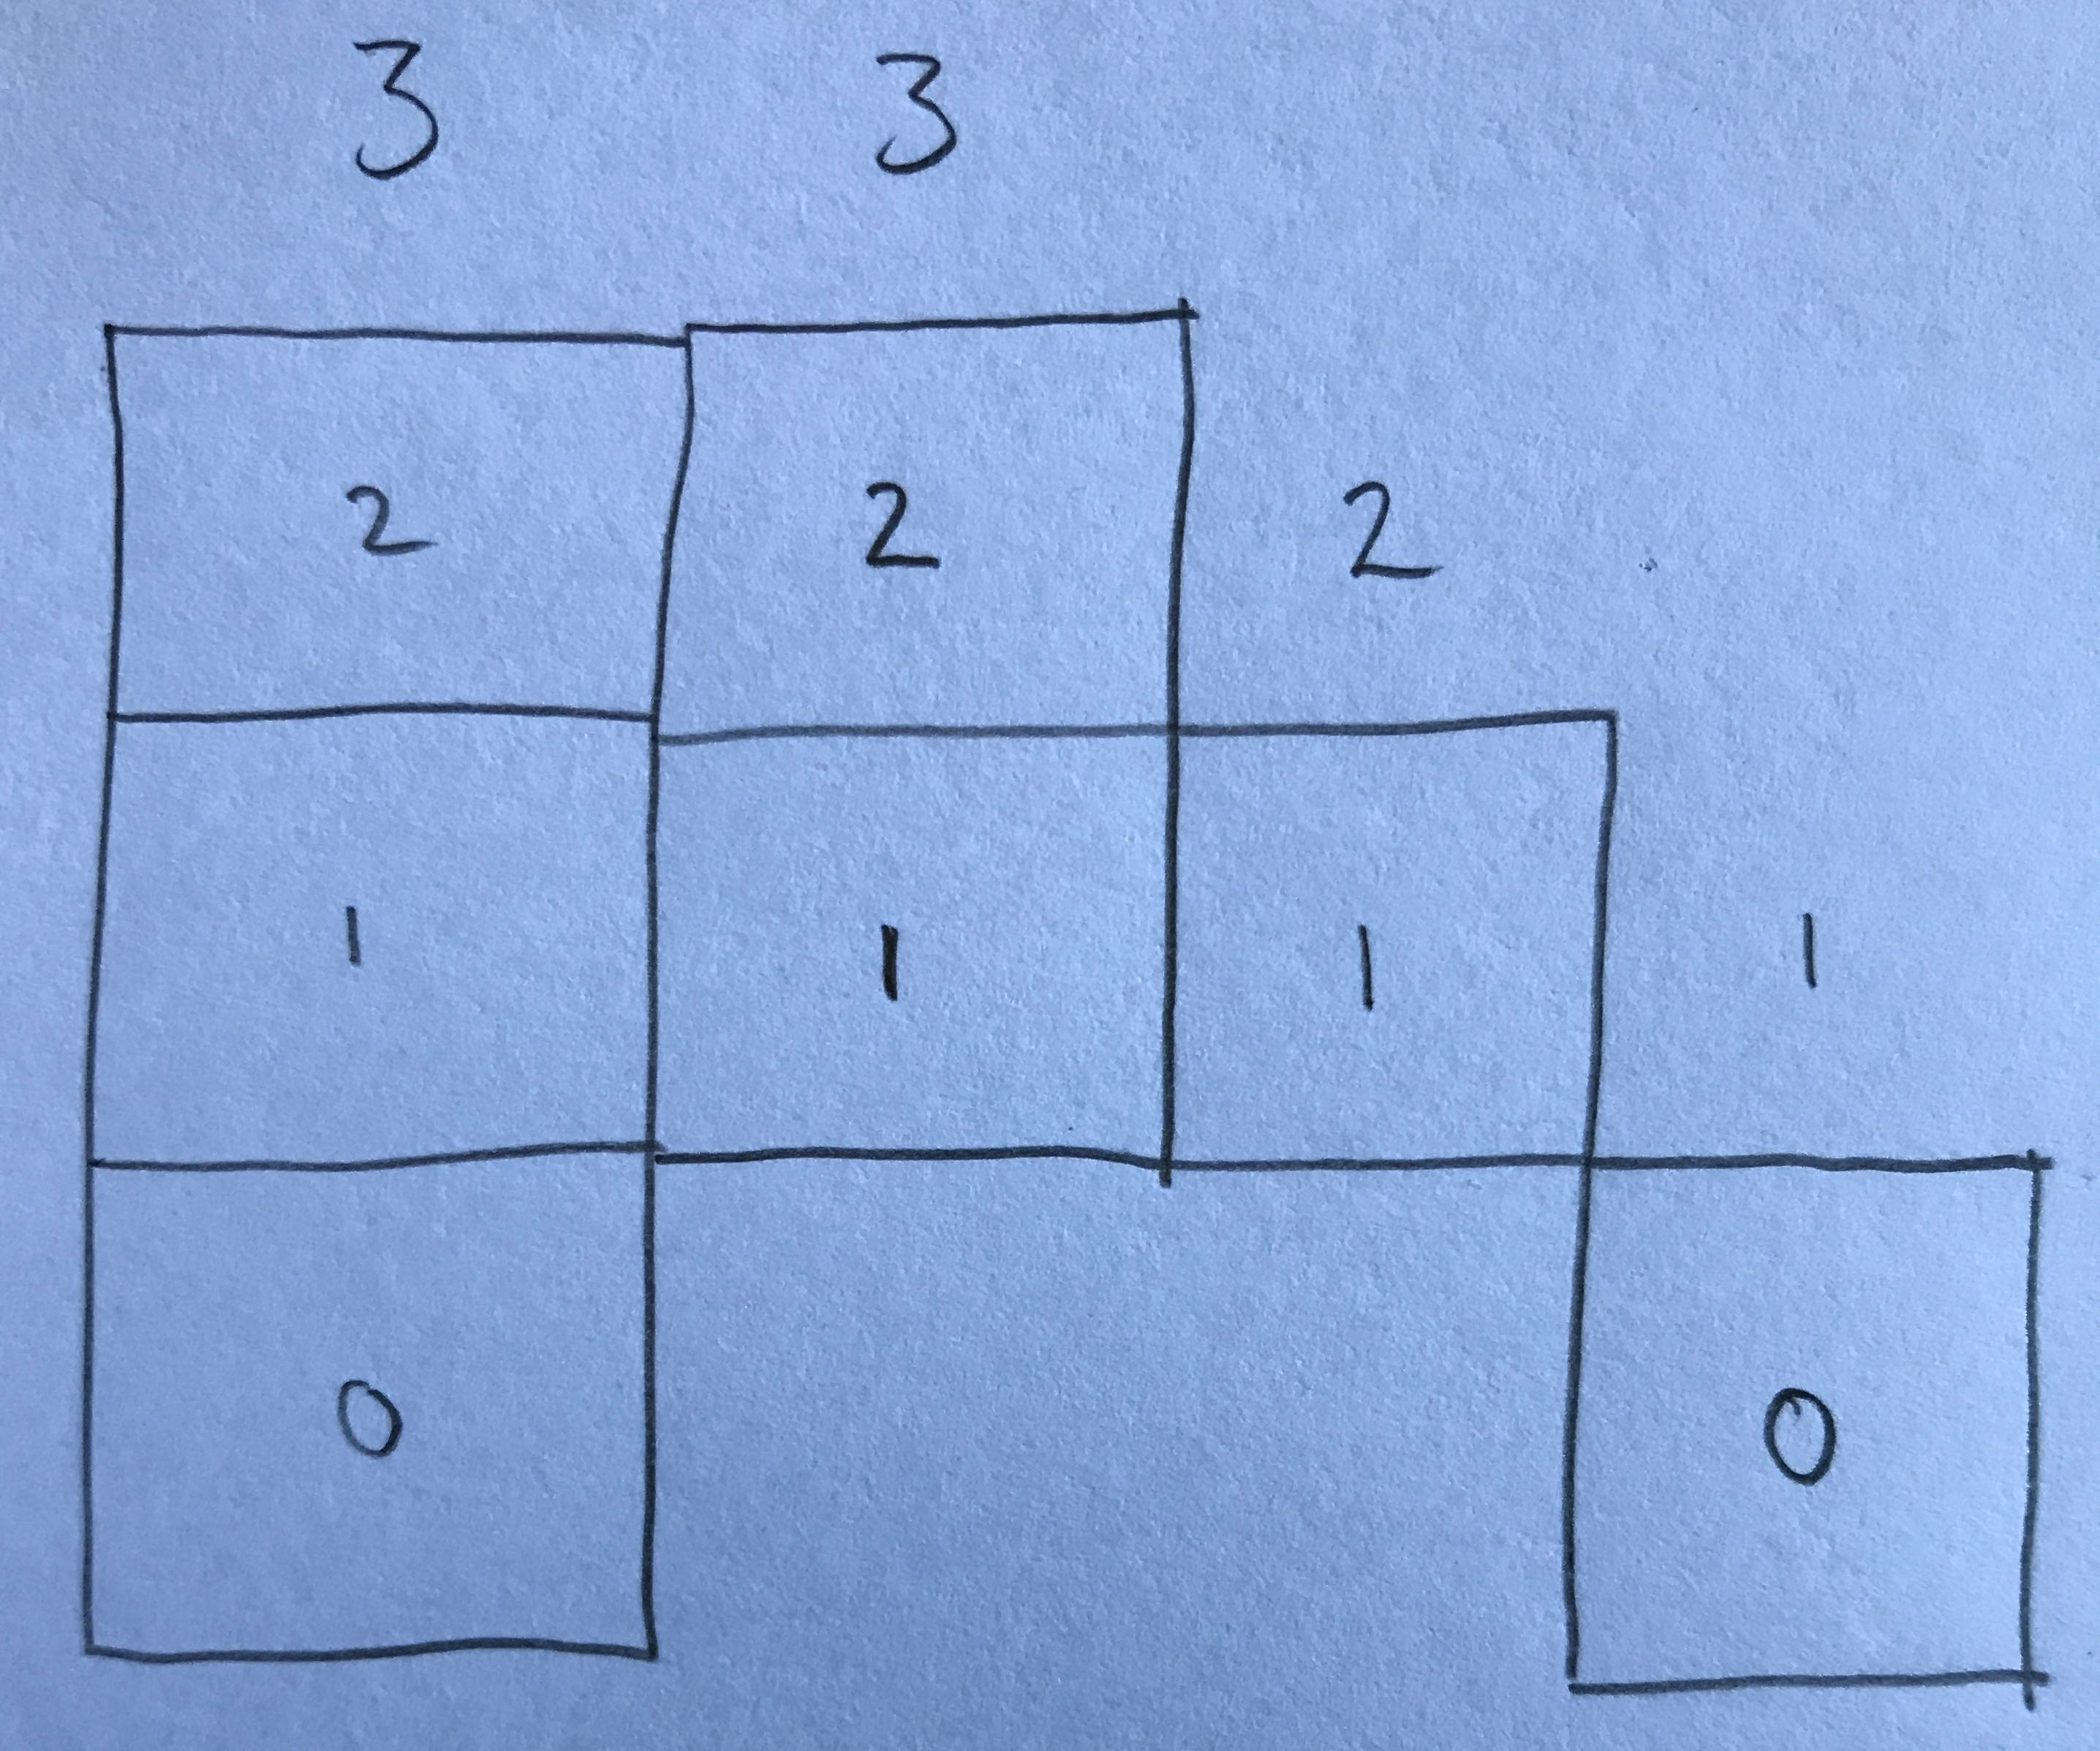
\includegraphics[width=\textwidth]{topology-2d-cells}}
      \only<3>{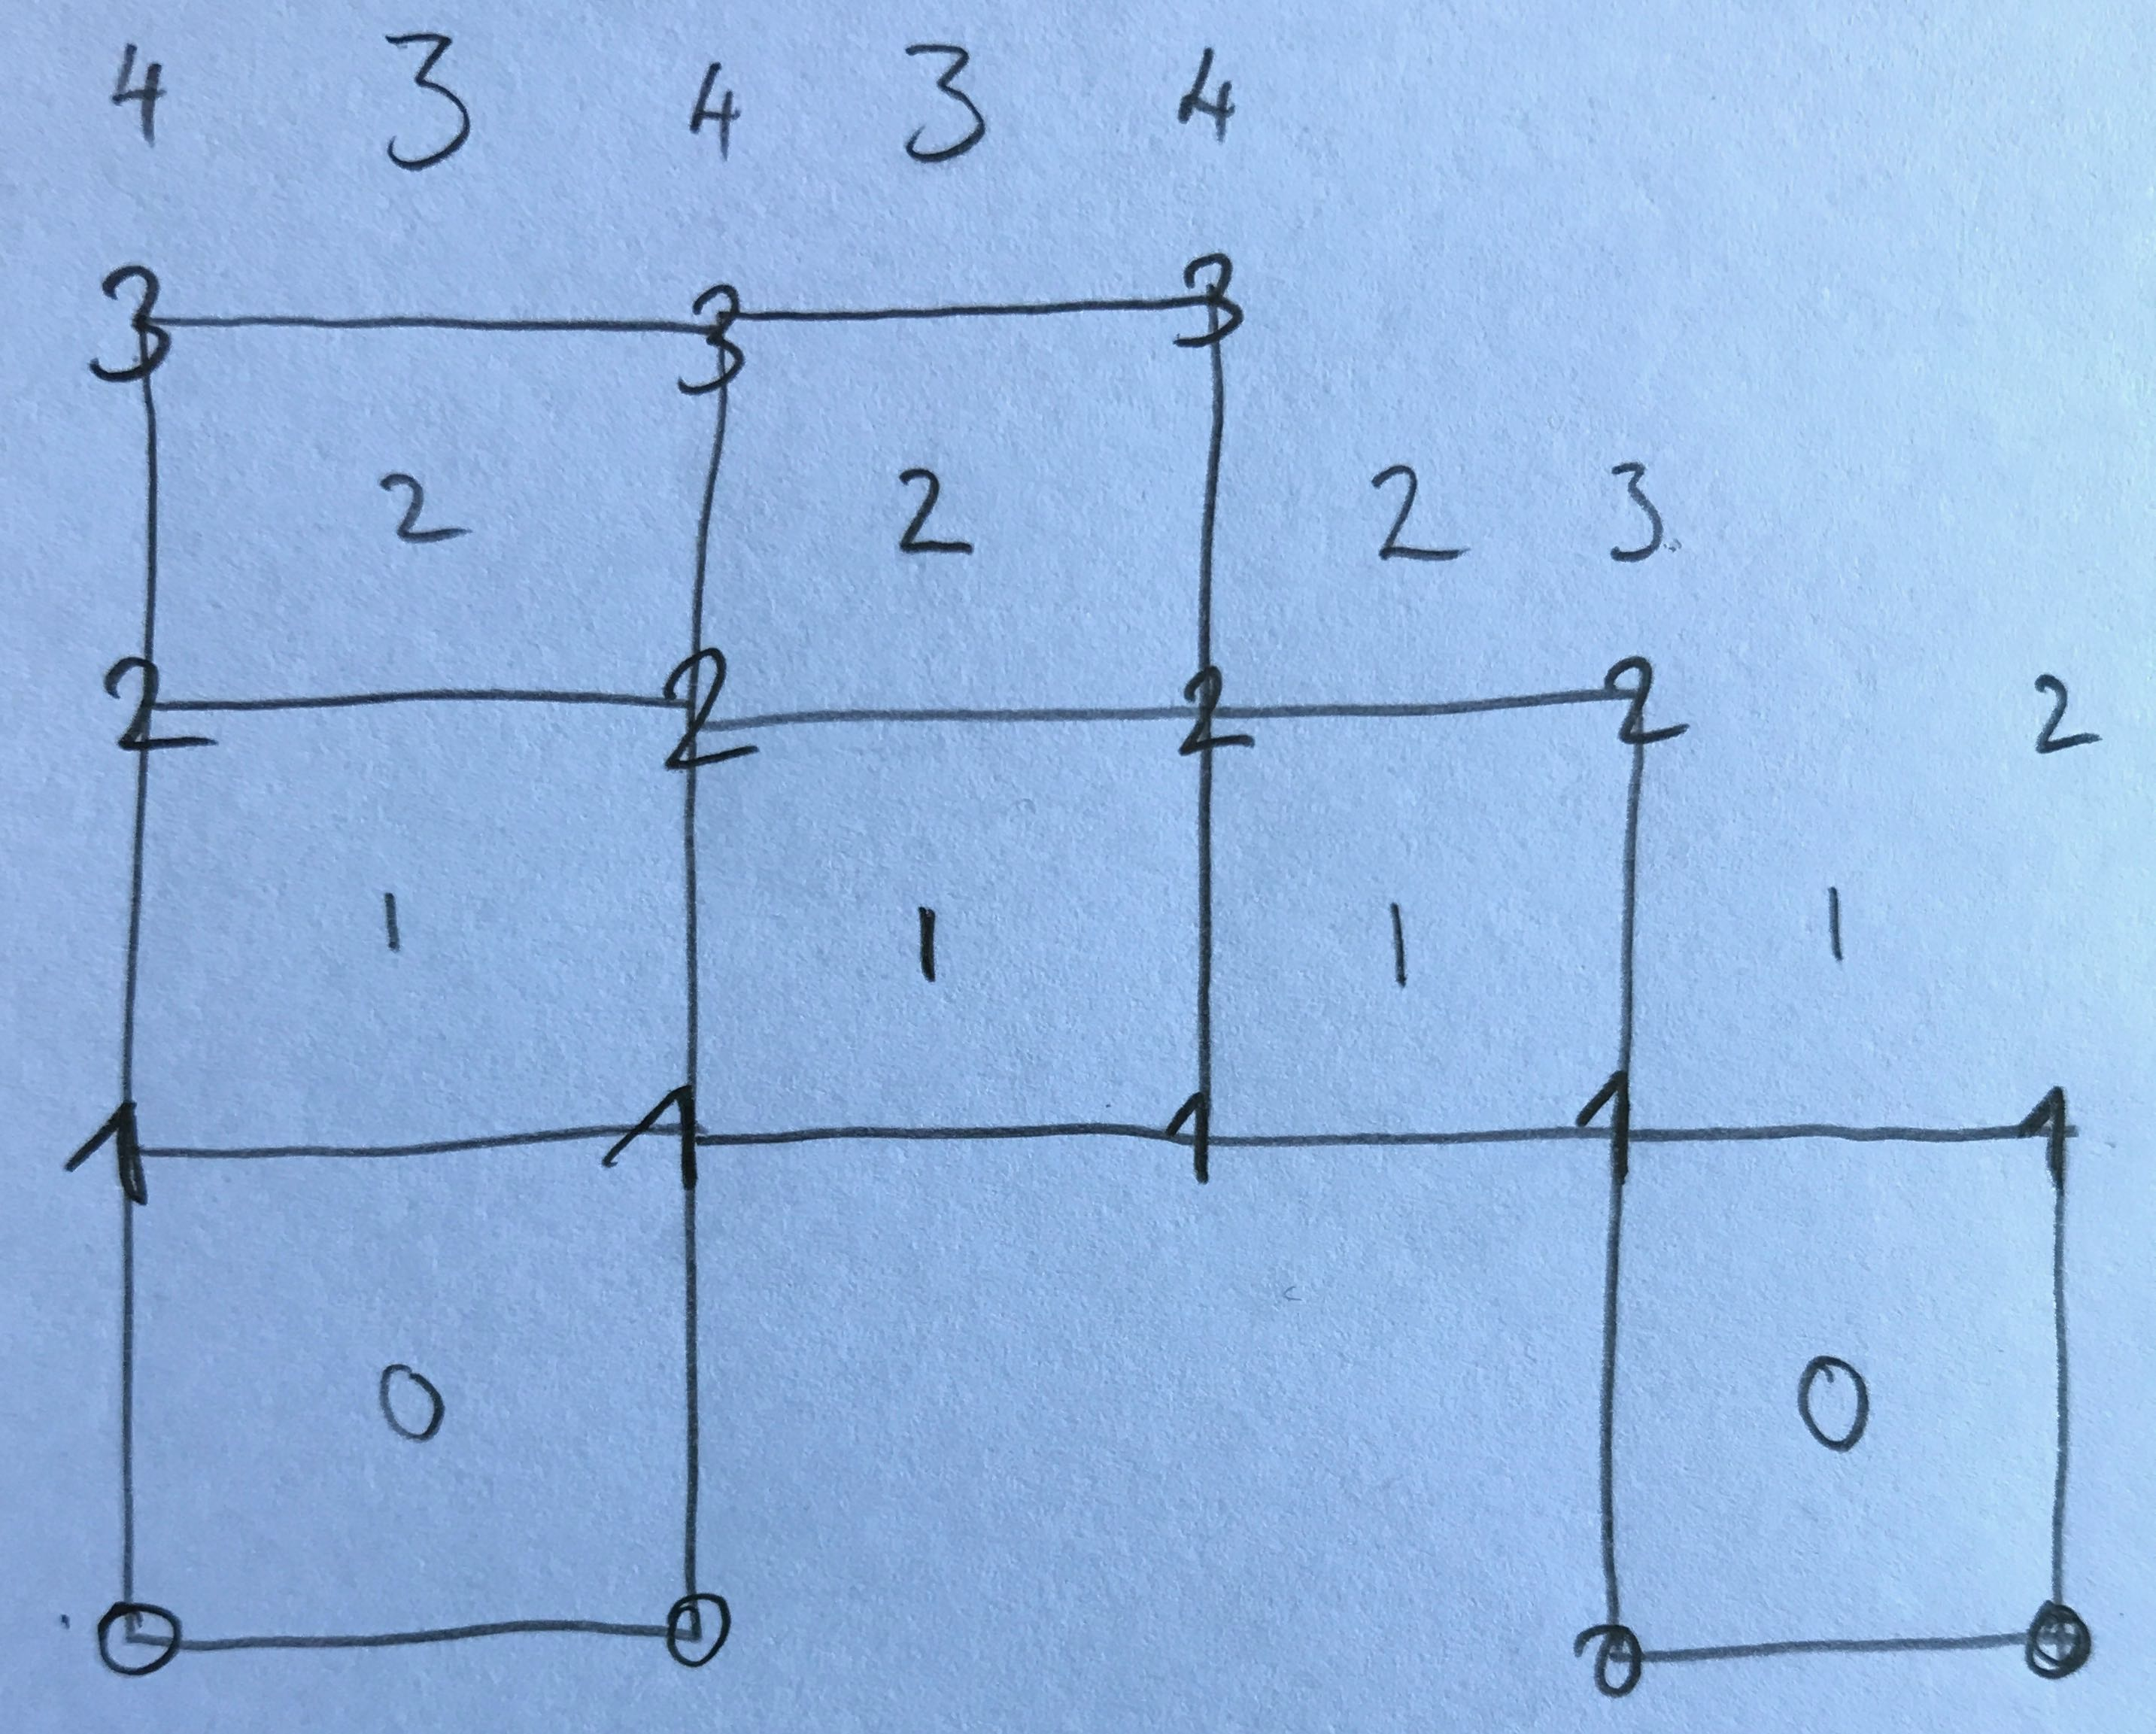
\includegraphics[width=\textwidth]{topology-2d-vertices}}
      \only<4>{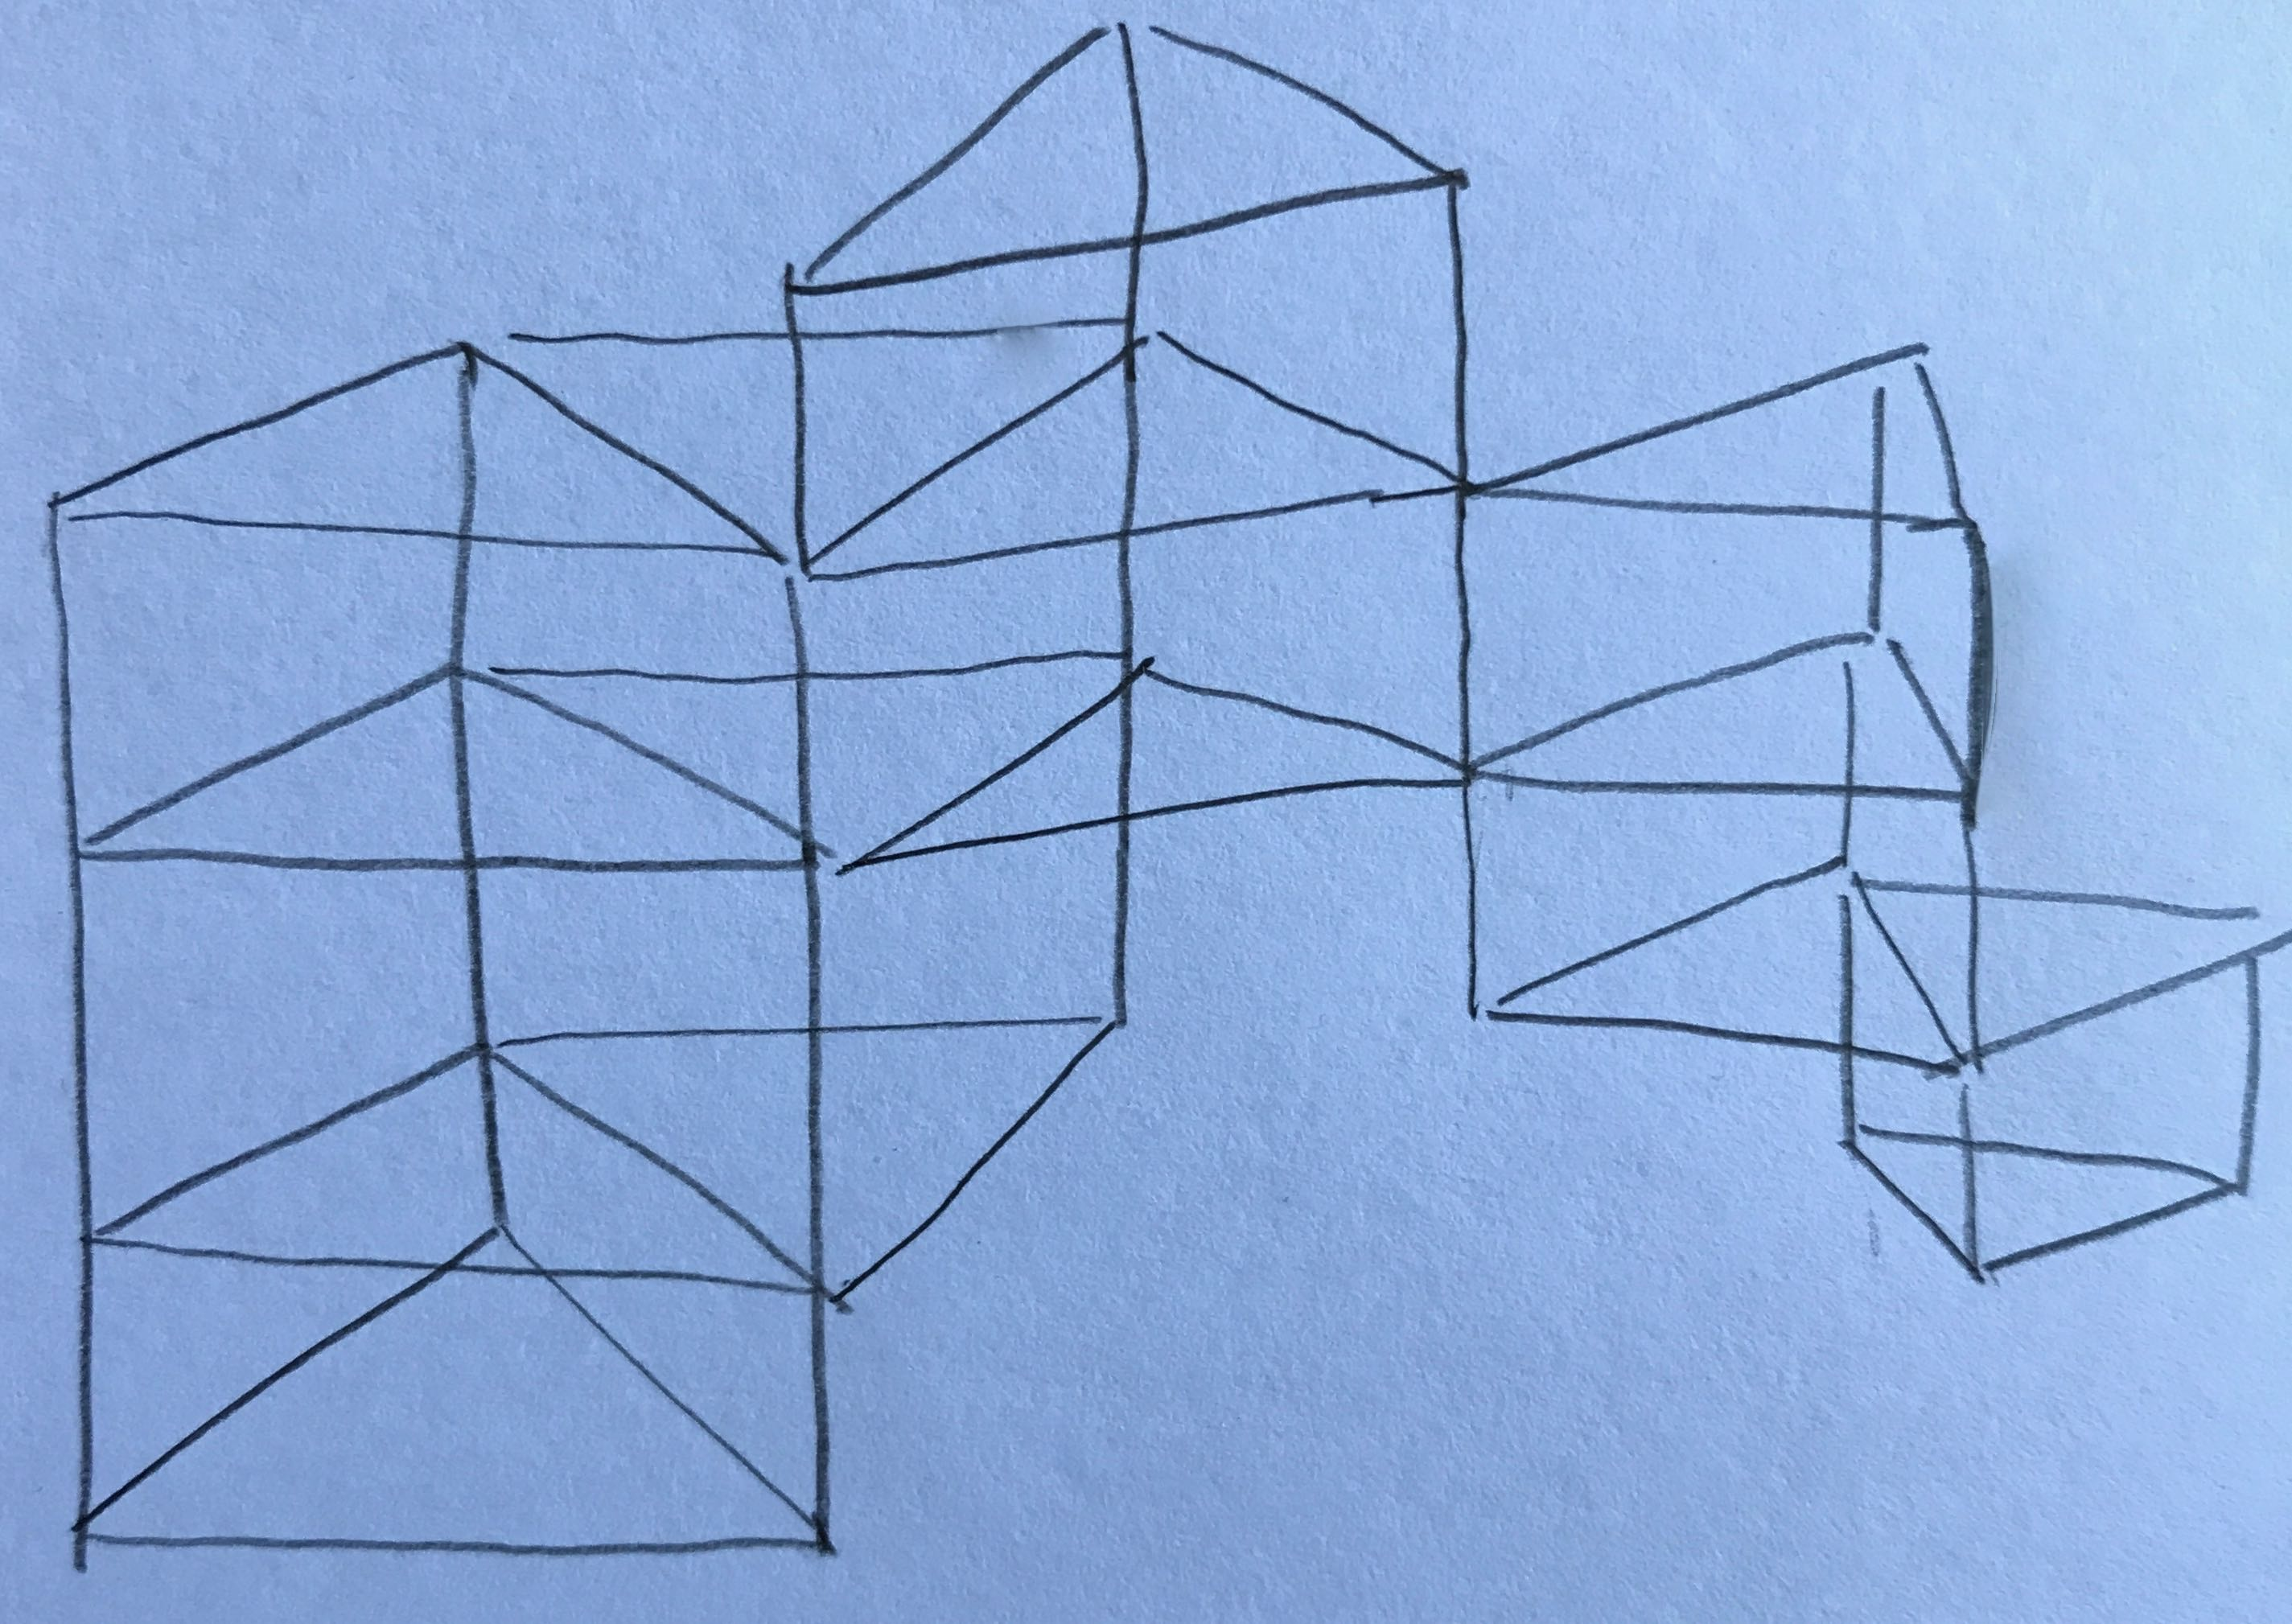
\includegraphics[width=\textwidth]{topology-3d}}
    \end{column}
  \end{columns}
\end{frame}

\begin{frame}[fragile]
  \frametitle{Datatype extension}
Iteration sets need \emph{four} values per entry.
  \begin{columns}
    \begin{column}{0.5\textwidth}
      Before
\begin{minted}[fontsize=\tiny]{python}
cells = ExtrudedSet(ncell, layers=10)
efacets = ExtrudedSet(nefacet, layers=10)
ifacets = ExtrudedSet(nifacet, layers=10)
\end{minted}
    \end{column}
    \begin{column}{0.5\textwidth}
\begin{minted}[fontsize=\tiny]{python}
cells = ExtrudedSet(ncell, layers=[[0, 10, 0, 10], 
                                   [1, 10, 1, 10],
                                   ...,
                                   [13, 27, 13, 27]])
efacets = ExtrudedSet(nefacet, layers=[[0, 10, 0, 10],
                                       ...])
ifacets = ExtrudedSet(nifacet, layers=[[1, 10, 1, 9],
                                       ...])
\end{minted}
    \end{column}
  \end{columns}
\end{frame}
\begin{frame}[plain]
  \begin{columns}
    \begin{column}{\textwidth}
      \only<1>{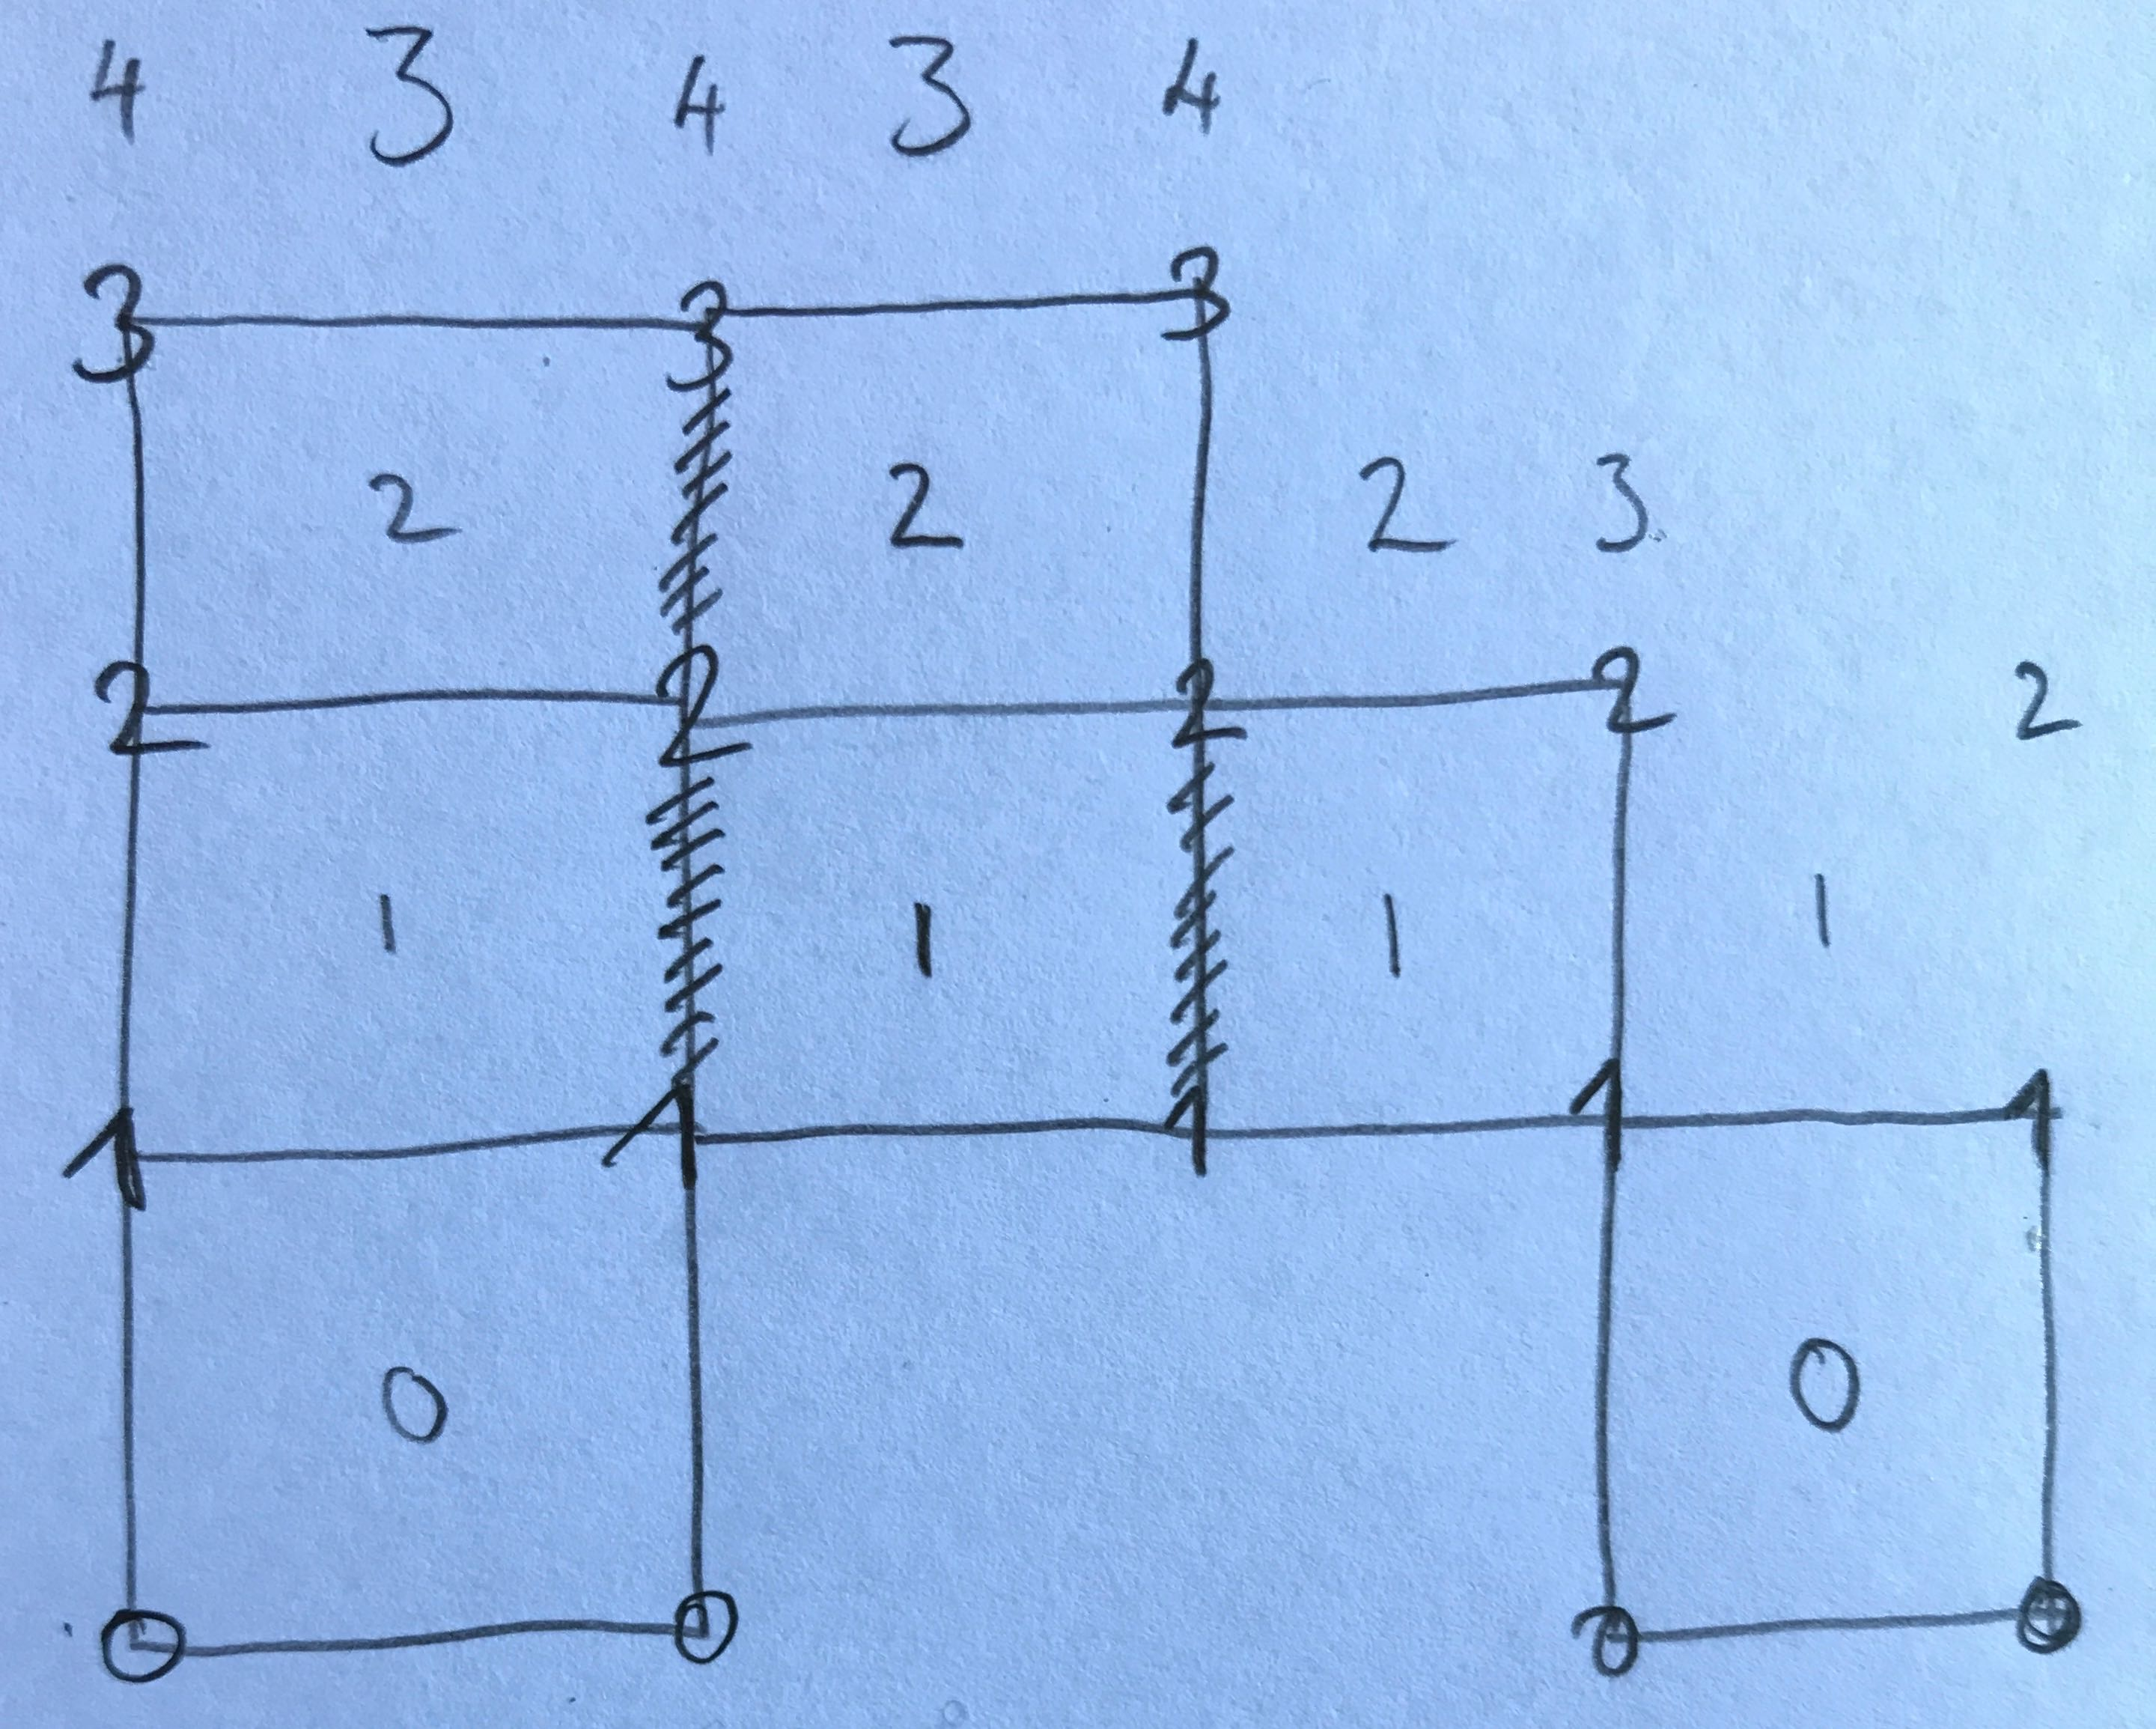
\includegraphics[width=\textwidth]{topology-2d-facets}}
    \end{column}
  \end{columns}
\end{frame}
\begin{frame}
  Preliminary support in Firedrake

  We squash interior facets geometrically, and then guarantee not to
  iterate over them.

  This creates degenerate cells, but maybe it's OK?  Unless the
  quadrature points fall on the edge (shouldn't).

  Could also do mixed cell shapes?  Now you have to worry about what
  happens to kernels.

  In any case, kernels need to have runtime-variable layer number.
\end{frame}


\end{document}
